% !TEX encoding = UTF-8 Unicode
% !BIB TS-program = biber

% This file is MIT-Thesis.tex, a LaTeX template for formatting an MIT thesis with the mitthesis class.
%
% Version: 1.17, 2024/11/02
%
% Author: John H. Lienhard, copyright 2024. Reuse under the MIT license: https://ctan.org/license/mit 

% Documentation is here: https://ctan.org/pkg/mitthesis

%% Don't modify the \DocumentMetadata command unless you know what it does. 
%% If this command throws an "undefined" error, your latex system is out of date: try commenting this command out.
\DocumentMetadata{
	lang		= en-US,
	pdfversion  = 1.7,
	pdfstandard = a-2b,
%	 pdfversion  = 2.0,
%    pdfstandard = a-4,
%	 debug		= {xmp-export}, % creates and xmpi file useful for checking metadata
}

%%%%%%%%%%%%%%%%%%%%%%%%%%%%%%%%%%%%%%%

\documentclass[twoside]{mitthesis}% fontset=newtx, fontset=libertine, fontset=libertinus, fontset=lmodern, fontset=newtx-sans-text, fontset=fira-newtxsf, fontset=heros-stix2, fontset=stix2, fontset=lmodern
%
% option [twoside]		gives facing-page behavior for printing; omitting twoside will eliminate even-numbered blank pages.
% option [lineno]	 	provides line numbers, as for editing
% option [mydesign] 	loads packages for color, title and list formats, margins, or captions: edit mydesign.tex to change defaults.
% option [fontset] is a keyvalue which can be:
%					 	for pdftex or unicode engines:  defaultfonts, libertine, libertinus, lmodern, lucida
%					 	for pdftex only: 				fira-newtxsf, newtx, newtx-sans-text
%						for unicode engines (luatex):	heros-stix2, stix2, termes, termes-stix2
%					 	if no key value is given, fonts default to CMR (pdftex) or LMR (unicode), i.e., "the LaTeX font".
%					 	You can edit the fontset files or you can write your own, myfonts.tex, and do [fontset=myfonts].
%						If you are using multiple languages, load the babel package in your fontset file, before the fonts.

%%%%%%%%% Packages used in sample chapters (not otherwise required) %%%%%%%

%% Package for code listing in Appendix A.
\usepackage{listings}%   documentation is here https://ctan.org/pkg/listings

%% Set chemical formulas nicely
\usepackage[version=4]{mhchem}%   documentation at https://ctan.org/pkg/mhchem

%% Latin filler used in Chapter 1, with a test for package version date (https://ctan.org/pkg/lipsum)
\usepackage{lipsum}
\IfPackageAtLeastTF{lipsum}{2021/09/20}{\setlipsum{auto-lang=false}}{}

%% Table related packages  

\usepackage{booktabs}% publication quality tables (https://ctan.org/pkg/booktabs)

\usepackage{array}% Additional options for column formats (https://ctan.org/pkg/array)

\usepackage{dcolumn}% For alignment of numbers on the decimal place (https://ctan.org/pkg/dcolumn) 
  \newcolumntype{d}[1]{D{.}{.}{#1}}% use with dcolumn package. Note: dcolumns are set in math mode.
  % syntax: d{x.y} where x is max number of digits before decimal and y is max number after.

% Package for multipage table in Appendix B.
\usepackage{longtable}% typeset multi-page tables (https://ctan.org/pkg/longtable)

%\usepackage{tabularx}% adjustable-width columns in tabular (https://ctan.org/pkg/tabularx)


%% Package for improved typography

\usepackage{microtype}% typographic fine-tuning, used in sample thesis committee page, but also acting globally on the text 


%%%%%%%%%  Graphics path (to figure files)  %%%%%%%%%%%%%%%%%%%%%%%%%%%%%%%%

%% Can set graphicspath to point to specific directories containing figures (the current directory is searched automatically)
%% For instance, to search a subdirectory of the current directory called "figures" and a parallel directory called "art", set:

% \graphicspath{ {figures/} {../art/} }% For details see: https://latexref.xyz/dev/latex2e.html#g_t_005cgraphicspath


%%%%%%%%%  Representative set-up for biblatex  %%%%%%%%%%%%%%%%%%%%%%%%%%%%%

%% Numerical citations of references
\usepackage[style=ext-numeric-comp,giveninits=true,maxbibnames=10,sorting=none]{biblatex}
 
%% IEEE style citations and references
% \usepackage[style=ieee,maxbibnames=10,sorting=none]{biblatex}% style=ext-numeric-comp,articlein=false,giveninits=true
%	 \DefineBibliographyStrings{english}{url= \textsc{url} ,  }% replaces the IEEE default "[Online]. Available" by "URL"

%% author-year style citations and references 
%% use \parencite, not \cite, when you want "(Author, year)"
%% The sample files are not set up to include parentheses.
% \usepackage[style=authoryear, maxbibnames=10]{biblatex} 


\addbibresource{mitthesis-sample.bib}%% <== change to YOUR bib file <= CHANGE

%% to avoid split urls and stretched white space, you can set the bibliography ragged-right:
%\appto{\bibsetup}{\raggedright}

%% biblatex is very powerful, and you can customize most aspects the reference list and citations to suit your needs.
%%   documentation is here: https://ctan.org/pkg/biblatex
%%   cheat sheet is here:   https://tug.ctan.org/info/biblatex-cheatsheet/biblatex-cheatsheet.pdf 

%% To ensure citations are set, run Latex --> biblatex/biber --> Latex again

%%%%%%%%%%  Option to use natbib   %%%%%%%%%%%%%%%%%%%%%%%%%%%%%%%%%%%%%%%%%

%\RequirePackage[numbers,sort&compress]{natbib}
 
%%% add bibliography to table of contents
%\apptocmd{\bibliography}{\addcontentsline{toc}{chapter}{\protect\textbf{\bibname}}}{}{}

%%% You can use this to rename the bibliography section
%\renewcommand{\bibname}{References}

%%% To adjust space between bibliography items 
%\setlength\bibsep{4pt plus 1pt minus 1pt}
%   change 4pt to something else; don't drop last two lengths (they are stretchable "glue")


%%%%%%%%%%  Option for "double spacing" %%%%%%%%%%%%%%%%%%%%%%%%%%%%%%%%%%%%

%% Back in the typewriter era, double spaced lines were convenient for editing with a pencil. 
%% In typography, the separation between lines is called "leading", and it is usually set in 
%% proportion to the font size (i.e., when the font is loaded).  If you really feel the need 
%% to change the line separation, the most attractive results will be obtained by changing the
%% leading in proportion to the the current font size, rather than just doubling the space.

%% The setspace package provides a tool for changing line separation. Use these two commands here:
%
% \usepackage{setspace}%  documentation at https://ctan.org/pkg/setspace
% \setstretch{1.1}% you can choose some other value for the stretch of space between lines
%
%% Use one or more of the these commands *AFTER* the frontmatter
%
% \onehalfspacing
% \doublespacing
% \singlespacing  % will turn these effects off (you can use these anywhere in the document)

%% The best result is usually to stay with leading selected by the typographer who set up the font.


%%%%%%%%%%%  Metadata  %%%%%%%%%%%%%%%%%%%%%%%%%%%%%%%%%%%%%%%%%%%%%%%%%%%%%%%

% Most of the document metadata is created automatically. 
% The following items should be adjusted to match your work. <================= !!!!!!!!!!

\hypersetup{%
	pdfsubject={Template for writing MIT theses with the mitthesis class},
	% Change this to briefly state topic of your thesis 
% 
	pdfkeywords={Göttingen, Neuroinformatics},
	% Add keywords that will help search engines and libraries to find your work.
	% Includes the name[s] of the author[s] 
	% (If you used \DocumentMetadata at line 14, you can just put "\CopyrightAuthor," for the names.)
%
	pdfurl={},
	% If you have a url for the thesis, put it here. Otherwise delete this.
	% (MIT Libraries will put your thesis in DSPACE with a persistent url after you submit it.)
%	
	pdfcontactemail={},
	% You can put a [permanent] email address into the metadata, if you like.
	% Otherwise delete this.
%
	pdfauthortitle={},
	% If you have a title, you can include it here.
}

%%%%%%%%%%%%  Math operators %%%%%%%%%%%%%%%%%%%%%%%%%%%%%%%%%%%%%%%%%%%%%%%%%%%%

% These commands declare two math operators, \erf{..} and \erfc{..} using mathtools
% note: * form produces automatic delimiter scaling; optional argument sets size manually, e.g. [\bigg]
% See Table 1.1 in Chapter 1

\DeclareMathOperator{\Erf}{erf}
\DeclareMathOperator{\Erfc}{erfc}
\DeclarePairedDelimiterXPP\erf[1]{\Erf\mkern1mu} (){}{#1}% increase to 2mu with stix2 font
\DeclarePairedDelimiterXPP\erfc[1]{\Erfc\mkern1mu} (){}{#1}


%%%%%%%%%%%%%%  End preamble %%%%%%%%%%%%%%%%%%%%%%%%%%%%%%%%%%%%%%%%%%%%%%%%%%%%%%%%%%%%%%%%%%%%%
%%%%%%%%%%%%%%%%%%%%%%%%%%%%%%%%%%%%%%%%%%%%%%%%%%%%%%%%%%%%%%%%%%%%%%%%%%%%%%%%%%%%%%%%%%%%%%%%%%

\begin{document}
%%% edit the following commands to match your thesis %%%%%%%%%%

\title{Influence of data diversity in brain decoding: An empirical study of image reconstruction from fMRI data}

% \Author{Author full name}{Author department}[Author's first PREVIOUS degree][Author's second PREVIOUS degree][...
% Note that third, fourth, fifth, and sixth arguments are optional [] and may be omitted

% note on names: most of the following names are made up; Silas Holman was a physics professor at MIT in the 19th century.

\Author{Matthias K. Mildenberger}{Department of Computer Science}
% \Author{Luisa Hernández}{Department of Research}[B.S. Mechanical Engineering, UCLA, 2018][M.S. Stellar Interiors, Vulcan Science Academy, 2020]
% \Author{Thurston Howell III}{Department of Economics}[MBA, Ferengi School of Management, 2022]

% Use once for each degree fulfilled by thesis
% For two degrees from one department, leave the department argument blank for the second degree {}.
\Degree{Master of Science in Applied Computer Science}{Department of Computer Science}
%\Degree{Master of Science in Physics}{}
%\Degree{Bachelor of Science in Mechanical Engineering}{Department of Mechanical Engineering}

% If there is more than one supervisor, use the \Supervisor command for each.
\Supervisor{Yoshihiro Nagano}{Assistant Professor of Neuroinformatics}
% \Supervisor{Edward C. Pickering}{Professor of Physics, and \\ \> Professor of Something Else}
% \Supervisor{Secunda Castor}{Professor of Research}
% \Supervisor{Quintus Castor}{Professor of Log Dams}

% Professor who formally accepts theses for your department (e.g., the Graduate Officer, Professor Sméagol,...)
% If more than one department, use more than once
\Acceptor{Tertius Castor}{Professor of Log Dams}{Graduate Officer, Department of Research} % \\ \> Third title}

% \Acceptor{Quarta Castor}{Professor of Lodge Building}{Graduate Officer, Department of Mechanical Engineering}
%%%  If you need to reduce vertical space, put the acceptor title in the second argument and leave the third blank, {}.
% \Acceptor{Primus Castor}{Professor and Undergraduate Officer, Department of Physics}{}

% Usage: \DegreeDate{Month}{year}
% Valid degree months are February, May, June, or September
\DegreeDate{May}{2025}

% Date that final thesis is submitted to department
\ThesisDate{May 01, 2025}


%%%%%%  Choose whether to have a CREATIVE COMMONS License  %%%%%%%%%%%%%%%%%%%%%%%%%%%%%%%%%%%%%%
%
% If you are using a cc license, uncomment the following line and insert details of your cc license here.
%
% \CClicense{CC BY-NC-ND 4.0}{https://creativecommons.org/licenses/by-nc-nd/4.0/}
%

%%%%%%%  Solutions for overflowing titlepage  %%%%%%%%%%%%%%%%%%%%%%%%%%%%%%%%%%%%%%%%%%%%%%%%%%%

% If your title page is overflowing (from too many names, degrees, etc.):
%
% (a) you can reduce the 12pt and 18pt skips between various blocks to 6pt with this command:
%
% \Tighten
%
% (b)  you can scale down the Signature block at the bottom with this command:
%
% \SignatureBlockSize{\small}  %or this one \SignatureBlockSize{\footnotesize}
%
% (c) you can put the acceptor name and title onto two lines, rather than three like this:
%
% \Acceptor{Tertius Castor}{Professor and Graduate Officer, Department of Research}{}
%
% (d) you can change the font size of the author name[s] with
%
%	\AuthorNameSize{\normalsize}
%
% (e) and you can omit any previous degrees from the title page, instead mentioning them in the biographical sketch

% Also, if you prefer to keep the text toward the top of the page with most white space at the bottom, you
% can use this command to squash all of the vertical glue (stretchy space) with this command:
%
% \Squash 
%
% This command is useful when the text has not already reach the bottom of the page, since the glue gets squashed automatically
% when the page is too full.

%%%%%%%%%%%%%%%%%%%%%%%%%%%%%%%%%%%%%%%%%%%%%%%%%%%%%%%%%%%%%%%%%%%%%%%%%%%%%%%%%%%%%%%%%%%%%%%%%

%%% Make titlepage
\maketitle

%%%%%%%%% Contents that you need to write follows! %%%%%%%%%%%%%%%%%%%%%%%%%%%%%%%%%%%%%%%%%%%%%% 

% \includeonly{acknowledgments,biography,chapter1,chapter2,...,appendixa,...} 
%   for usage of includeonly, see https://latexref.xyz/_005cinclude-_0026-_005cincludeonly.html

%%% Frontmatter (write this material in the mentioned files)  %%%%%%%%%%%%%%%%%%%%%%%%%%%%%%%%%%%

% This page is optional. Edit the file committee_members.tex 
% % Sample thesis committee page for mitthesis.cls
% Version 1.01, 2024/10/08
%
% This page is not required by the MIT Libraries, but some departments require it.
%
% Insert between title page and abstract page.
% Format this page in any way that you like.  
% Add supervisor titles, degrees, and departments as appropriate.

%%%%% FORMATTING COMMANDS %%%%%%%%%%%%%%%%%%

%% Format title
\NewDocumentCommand\CommitteePageTitle{m}{
	\vspace*{75pt}%36pt}
	\IfPackageLoadedTF{microtype}
		{\textls*{\Large\textbf{\MakeUppercase{#1}}}}
		{{\Large\textbf{\MakeUppercase{#1}}}}%
	\pdfbookmark[0]{#1}{Committee}%
	\vspace*{10pt}%
}
% \textls* produces additional letter separation (appropriate for capitalized display text),
% PROVIDED THAT \usepackage{microtype} has been loaded in the preamble. 
% The extra space added is 100/1000 em (adjustable, see package documentation).

%% Format committee member subheadings
\NewDocumentCommand\Role{m}{
	\vspace*{50pt}%25pt}
	\IfPackageLoadedTF{microtype}
		{\textls*{\large{\textsc{#1}}}}
		{{\large\textsc{#1}}}%
	\vspace*{12pt}%
}

%%%%%%%%%%%%%%%%%%%%%%%%%%%%%%%%%%%%%%%%%%%%%

\begin{flushright}

\CommitteePageTitle{Thesis committee}

\Role{  }

 \textbf{Marcus Gavius Apicius} \\
 {\itshape
 Professor of Cooking Arts \\
 Department of Food Science \\
 }

\Role{Thesis Readers}

 \textbf{Marie-Antoine Carême} \\
 {\itshape
   Professor of Haute Cuisine \\
   Department of Food Science \\[18pt]
 }

 \textbf{Julia Child}\\
 {\itshape
   Professor of French Cuisine \\
   Department of Food Science \\[18pt]
 }

 \textbf{Miles Gloriosus} \\
 {\itshape
   Professor of Personal Pronouns \\
   Department of Rhetoric \\
 }

\end{flushright}

\cleardoublepage


% The abstract environment creates all the required headings and footers. 
% You only need to the text of the abstract in the file abstract.tex
\begin{abstract}
	% From mitthesis package
% Version: 1.01, 2023/06/19
% Documentation: https://ctan.org/pkg/mitthesis
%
% The abstract environment creates all the required headers and footnote. 
% You only need to add the text of the abstract itself.
%
% Approximately 500 words or less; try not to use formulas or special characters
% If you don't want an initial indentation, do \noindent at the start of the abstract

\noindent{}Reconstructing images directly from human brain activity was once considered science fiction; today, brain decoding using functional magnetic resonance imaging (fMRI) is turning this concept into reality. However, current methods lack the ability to properly reconstruct concepts that are not present in the training data. Recent findings in the field have shown that increasing the dimensions and thus the diversity of the training data may lead to better generalisation to unknown concepts. In this paper, three experiments are conducted to investigate the influence of training data diversity on the generalisation of image reconstruction algorithms and the ability to reconstruct images that are dissimilar to the training data. In the first experiment, diversity-based subsampling of the training data was performed to outperform a random subsampling baseline. In the second experiment, image captions were generated to emphasise the low-level (shape, colour) features of the training images, by using this approach the reconstruction of out-of-distribution (OOD) data could be improved. In the third experiment, perturbations were used to either increase or decrease the semantic value of the training data, the results of this experiment were inconclusive. In conclusion, the three experiments showed that the diversity of the dataset can play an important role in helping image reconstruction to generalise to unfamiliar concepts. Further research is needed to find the essential image dimensions needed in the data to create a universal image reconstruction method. It is also important to investigate how these dimensions correspond to the elicited brain activity.

% Yet, the accuracy of these reconstructions critically depends on the diversity of visual stimuli presented during training. This thesis explores how varying the richness and variety of training images influences the brain decoding process and ultimately determines the quality of reconstructed visual experiences.% use \input rather than \include because we're inside an environment
\end{abstract}

% %% acknowledgments.tex

% From mitthesis package
% Version: 1.02, 2024/06/19
% Documentation: https://ctan.org/pkg/mitthesis

\chapter*{Acknowledgments}
\pdfbookmark[0]{Acknowledgments}{acknowledgments}


I would like to express my deepest gratitude to my supervisor, Yoshihiro Nagano, for his excellent guidance throughout this work. His insigthful feedback, support in exploring and refining ideas and the thoughtful comments have been invaluable for me. Especially during times when the results did not align with my expectations he was able to motivate me and always find a new angle to view at the problems that eventually enabled me to make the next step forward. 

I would also like to thank Prof.\ Florentin Wörgötter for taking the role of second supervisor. Even though the topic was new to him, he was willing to support the work without hesitation. This gave me the unique opportunity to explore this interesting field. 

I also want to thank Linnéa Nöth for her support during the entire process. The engaging discussions, her help in structuring both my thoughts and the text, and encouragement during challenging moments kept me going. Thank you!

\section*{Software and Tools Used}

% Für diese Arbeit wurden diverse software und tools genutzt. Darunter die folgenden: Visual Studio Code als Editor für das Manuskript und den Programmcode, GitHub zur Versionierung des Manuskripts und des sourcecodes, Zotero zum Management der Literatur, LaTex zur Erstellung des fertigen Dokuments, ChatGPT zur Optimierung von Programmcode und der Diskussion von Formulierungen in der englischen Sprache, DeepL zur Übersetzung von der deutschen in die englische Sprache. Zusätzlich Google Scholar, Consensus.app und allen.ai paperfinder zur Literaturrecherche. 

Various software and tools were used in the course of this work, including the following: Visual Studio Code as the editor for both the manuscript and source code, GitHub for version control, Zotero for literature management, and LaTeX for compiling the final document. Additionally, ChatGPT was used to optimize programming code and to discuss English phrasings, DeepL supported translations from German into English. For literature research, Google Scholar, Consensus.app, and the Allen.ai PaperFinder were used. The exact libraries that have been used for the programming part of this thesis are listed in the according requirements of the conda environment in the GitHub repository of this work. 
% acknowledgments.tex (.tex extension is presumed by \include) 

% %% biography.tex
%% This section is optional

% From mitthesis package
% Version: 1.02, 2024/06/19
% Documentation: https://ctan.org/pkg/mitthesis

\chapter*{Biographical Sketch}
\pdfbookmark[0]{Biographical Sketch}{biosketch}


Silas Whitcomb Holman was born in Harvard, Massachusetts on January 20, 1856. He received his S.B. degree in Physics from MIT in 1876, and then joined the MIT Department of Physics as an Assistant. He became Instructor in Physics in 1880, Assistant Professor in 1882, Associate Professor in 1885, and Full Professor in 1893. Throughout this period, he struggled with increasingly severe rheumatoid arthritis. At length, he was defeated, becoming Professor Emeritus in 1897 and dying on April 1, 1900.

Holman's light burned brilliantly before his tragic and untimely death. He published extensively in thermal physics, and authored textbooks on precision measurement, fundamental mechanics, and other subjects. He established the original Heat Measurements Laboratory. Holman was a much admired teacher among both his students and his colleagues. The reports of his department and of the Institute itself refer to him frequently in the 1880's and 1890's, in tones that gradually shift from the greatest respect to the deepest sympathy.

Holman was a student of Professor Edward C. Pickering, then head of the Physics department. Holman himself became second in command of Physics, under Professor Charles R. Cross, some years later. Among Holman's students, several went on to distinguish themselves, including: the astronomer George E. Hale ('90) who organized the Yerkes and Mt. Wilson observatories and who designed the 200 inch telescope on Mt. Palomar; Charles G. Abbot ('94), also an astrophysicist and later Secretary of the Smithsonian Institution; and George K. Burgess ('96), later Director of the Bureau of Standards. % biography.tex (optional, see https://libraries.mit.edu/distinctive-collections/thesis-specs/#format)

%%% Table of contents and lists of stuff (delete unused lists, i.e., if no tables or figures) %%%%%

\tableofcontents
% \listoffigures
% \listoftables

%%% Chapters of thesis  %%%%%%%%%%%%%%%%%%%%%%%%%%%%%%%%%%%%%%%%%%%%%%%%%%%%%%%%%%%%%%%%%%%%%%%%%%%

%% If you want to use "double spacing", you should start here...

 % From mitthesis package
% Version: 1.07, 2024/09/26
% Documentation: https://ctan.org/pkg/mitthesis


\chapter{Introduction}

\lipsum[1-2] Postremo aliquos futuros suspicor, qui me ad alias litteras vocent, genus hoc scribendi, etsi sit elegans, personae tamen et dignitatis esse negent~\cite{DKE1969,ww1920,kirk2288a,churchill1948,gibbs1863}.

\section[A section discussing the first issue: \(J/\psi\)]{A section discussing the first issue: \ifpdftex\(\bm{J}/\bm{\psi}\)\else{\(\symbfit{J/\psi}\)}\fi}


We begin with some ideas from the literature \cite{Fong2015,sharpe1}. 
\begin{equation}\label{eqn:1}
\frac{\partial}{\partial t}\left[\rho\bigl(e + \lvert\vec{u}\rvert^2\big/2\bigr)\right]  + \nabla\cdot\left[\rho\bigl(h + \lvert\vec{u}\rvert^2\big/2 \bigr)\vec{u}\right]
 ={}-\nabla \cdot \vec{q} +  \rho \vec{u}\cdot\vec{g}+ \frac{\partial}{\partial x_j}\bigl(d_{ji}u_i\bigr)
\end{equation}
 \lipsum[3]

\lipsum[4] And more citations~\cite{sharpe1,GSL}.  Then we write some more and include our citations~\cite{Swaminathan2017IDABRO,dlmf,amsmath}. The configuration is shown in Fig.~\ref{fig:golden2}.

%%%%%%%%%%%%%%%%%  begin figure  %%%%%%%%%%%%%%%%%%%%%%%%%%%
\begin{figure}[t]
% sample images are from mwe package, but should be found by latex in the tex tree w/o loading that package
\begin{subfigure}[c]{0.495\textwidth}
\centering{\includegraphics[alt={sample image},width=0.99\textwidth]{example-image-c}}%
\subcaption{\label{fig:golden}}
\end{subfigure}
%%%%%%%% don't leave a break here
\begin{subfigure}[c]{0.495\textwidth}
\centering{\includegraphics[alt={sample image},width=0.99\textwidth]{example-image-c}}%
\subcaption{\label{fig:golden2}}%
\end{subfigure}%
\caption{A figure with two subfigures: (a) first subfigure; (b) second subfigure.\label{fig:4}}
\end{figure}
%%%%%%%%%%%%%%%%%%%  end figure  %%%%%%%%%%%%%%%%%%%%%%%%%%%%%

\lipsum[4]

%% note use of \ref* here to avoid placing a nested link in the table of contents
\subsection[Subsection~eqn.~(\ref*{eqn:WT1})]{Subsection~eqn.~\eqref{eqn:WT1}}
\lipsum[5-6]

\subsubsection{A subsubsection}
\lipsum[7]

\begin{equation}\label{eqn:WT1}
L(\ifpdftex\bm{A}\else\symbfup{A}\fi) = \begin{pmatrix}
\dfrac\varphi{(\varphi_1,\varepsilon_1)}			& 0 												 & \hdotsfor{3} 							& 0 \\[4\jot]
\dfrac{\varphi k_{2,1}}{(\varphi_2,\varepsilon_1)}	& \dfrac\varphi{(\varphi_2,\varepsilon_2)}			 & 0 										& \hdotsfor{2} & 0 \\[4\jot]
\dfrac{\varphi k_{3,1}}{(\varphi_3,\varepsilon_1)}	& \dfrac{\varphi k_{3,2}}{(\varphi_3,\varepsilon_2)} & \dfrac\varphi{(\varphi_3,\varepsilon_3)}	& 0 & \hdotsfor{1} & 0 \\[\jot]
\vdots 												&  													 &  & \smash{\rotatebox{15}{$\ddots$}} &  & \vdots \\[\jot]
\dfrac{\varphi k_{n-1, 1}}{(\varphi_{n-1},\varepsilon_1)}		& \dfrac{\varphi k_{n-1, 2}}{(\varphi_{n-1},\varepsilon_2)} & \hdotsfor{1} & 
	\dfrac{\varphi k_{n-1,n-2}}{(\varphi_{n-1},\varepsilon_{n-2})}	& \dfrac{\varphi}{(\varphi_{n-1},\varepsilon_{n-1})} 		& 0 \\[4\jot]
\dfrac{\varphi k_{n,1}}{(\varphi_n,\varepsilon_1)}				& \dfrac{\varphi k_{n,2}}{(\varphi_n,\varepsilon_2)}		& \hdotsfor{2}	&
	\dfrac{\varphi k_{n,n-1}}{(\varphi_n,\varepsilon_{n-1})} 		& \dfrac{\varphi}{(\varphi_n,\varepsilon_n)}
\end{pmatrix}
\end{equation}

\section{Description our paradigm}\label{ch1:theidea}

\lipsum[8] No dissertation is complete without footnotes.\footnote{First footnote. $a_h = F_m$ See section~\ref{sec:stratified-flow}.}\footnote{Another interesting detail.}\footnote{And another really important idea to have in mind~\cite{reynolds1958,clauser56,lienhard2020,johnson1980,johnson1965,mpl}.} 

\begin{figure}[t]
% sample image is from mwe package, but should be found by latex in the tex tree w/o loading that package
\centering\includegraphics[alt={sample image},width=6.67cm]{example-image-b} 
\caption{Caption text\label{example-image-b}~\cite{GSL}.}
\end{figure}


\subsection{Conversion to a metaheuristic}

\lipsum[11-12] This concept is discussed further in section~\ref{sec:stratified-flow}, and Refs.~\cite{euler1740,fourier1822}.



\section{Other generalizations}

\subsection{The most general case}

\lipsum[7] And another citation, so that our sources will be unambiguous~\cite{montijano2014}.
\begin{gather}
\ce{x Na(NH4)HPO4 ->[\Delta] (NaPO3)_x + x NH3 ^ + x H2O} \\[0.5em]
\ce{^234_90Th -> ^0_-1$\beta${} + ^234_91Pa} \\[0.5em]
\ce{SO4^2- + Ba^2+ -> BaSO4 v} \\[0.5em]
\ce{Zn^2+
<=>[+ 2OH-][+ 2H+]
$\underset{\textrm{amphoteric hydroxide}}{\ce{Zn(OH)2 v}}$
<=>[+ 2OH-][+ 2H+]
$\underset{\textrm{tetrahydroxozincate}}{\ce{[Zn(OH)4]^2-}}$
}
\end{gather}
These examples of chemical formul\ae\ are copied directly from the documentation of the \texttt{mhchem} package, which was used to typeset them.

\section{Baroclinic generation of vorticity\label{sec:stratified-flow}}

Substitution of the particle acceleration and application Stokes theorem leads to the \textit{Kelvin-Bjerknes circulation theorem}, for
$\rho \neq \textrm{fn}(p)$:
\begin{align}
\frac{d\Gamma}{dt} &{}= \frac{d}{dt} \int_{\mathcal{C}} \mathbf{u} \cdot d\mathbf{r}\\
				   &{}= \int_{\mathcal{C}} \frac{D\mathbf{u}}{Dt} \cdot d\mathbf{r} + \underbrace{\int_{\mathcal{C}} \mathbf{u}\cdot d\biggl( \frac{d\mathbf{r}}{dt}\Biggr)}_{=\, 0} \\[-2pt]
                   &{}= \iint_{\mathcal{S}} \nabla \times \frac{D\mathbf{u}}{Dt}  \cdot d\mathbf{A}\\
                   &{}= \iint_{\mathcal{S}}  \nabla p \times \nabla \left( \frac{1}{\rho}\right) \cdot d\mathbf{A}
\end{align}

Baroclinic generation of vorticity accounts for the sea breeze and various other atmospheric currents in which temperature, rather than pressure, creates density gradients. Further, this phenomenon accounts for ocean currents in straits joining more and less saline seas, with surface currents flowing from the fresher to the saltier water and with bottom current going oppositely.

%% Nomenclature list is optional
%
%  This environment takes three optional arguments:
%		[1] adjust space between symbol and definition
%		[2] name (heading) of the nomenclature list
%		[3] level - can be "section" or "chapter" depending on whether you
%			have one nomenclature list for whole thesis or one for each
%			chapter. 
\begin{nomenclature}[2em][Nomenclature for Chapter~1][section]
\EntryHeading{Roman letters}
\entry{$\mathcal{C}$}{material curve}
\entry{$\mathbf{r}$}{material position [m]}
\entry{$\mathbf{u}$}{velocity [m s$^{-1}$]}
\EntryHeading{Greek letters}
\entry{$\Gamma$}{circulation [m$^2$ s$^{-1}$]}
\entry{$\rho$}{mass density [kg m$^{-3}$]}
\end{nomenclature}

%%%%%%%%%%%%%%% begin table %%%%%%%%%%%%%%%%%% 
\begin{table}[t]
\caption{The error function and complementary error function}\label{tab:1}%
\centering{%
\begin{tabular*}{0.8\textwidth}{@{\hspace*{1.5em}}@{\extracolsep{\fill}}ccc!{\hspace*{3.em}}ccc@{\hspace*{1.5em}}}
\\[-0.5em]
\toprule
\multicolumn{1}{@{\hspace*{1.5em}}c}{$x$\rule{0pt}{8pt}} &
\multicolumn{1}{c}{$\erf{x}$} &
\multicolumn{1}{c!{\hspace*{3.em}}}{$\erf{x}$} &
\multicolumn{1}{c}{$x$} &
\multicolumn{1}{c}{$\erfc{x}$} &
\multicolumn{1}{c@{\hspace*{1.5em}}}{$\erfc{x}$} \\ \midrule
0.00 & 0.00000 & 1.00000 & 1.10 & 0.88021 & 0.11980 \\
0.05 & 0.05637 & 0.94363 & 1.20 & 0.91031 & 0.08969 \\
0.10 & 0.11246 & 0.88754 & 1.30 & 0.93401 & 0.06599 \\
0.15 & 0.16800 & 0.83200 & 1.40 & 0.95229 & 0.04771 \\
0.20 & 0.22270 & 0.77730 & 1.50 & 0.96611 & 0.03389 \\
0.30 & 0.32863 & 0.67137 & 1.60 & 0.97635 & 0.02365 \\
0.40 & 0.42839 & 0.57161 & 1.70 & 0.98379 & 0.01621 \\
0.50 & 0.52050 & 0.47950 & 1.80 & 0.98909 & 0.01091 \\
0.60 & 0.60386 & 0.39614 & 1.82\makebox[0pt][l]{14} & 0.99000 & 0.01000 \\
0.70 & 0.67780 & 0.32220 & 1.90 & 0.99279 & 0.00721 \\
0.80 & 0.74210 & 0.25790 & 2.00 & 0.99532 & 0.00468 \\
0.90 & 0.79691 & 0.20309 & 2.50 & 0.99959 & 0.00041 \\
1.00 & 0.84270 & 0.15730 & 3.00 & 0.99998 & 0.00002 \\
\bottomrule
\end{tabular*}
}%
\end{table}
%%%%%%%%%%%%%%%% end table %%%%%%%%%%%%%%%%%%% 

% .tex extension is presumed
% \include{chapter2}
% \include{chapter3}
% \include{chapter4}


%%% Appendicies of thesis  %%%%%%%%%%%%%%%%%%%%%%%%%%%%%%%%%%%%%%%%%%%%%%%%%%%%%%%%%%%%%%%%%%%%%%%%

% \appendix
% % From mitthesis package
% Version: 1.01, 2023/07/04
% Documentation: https://ctan.org/pkg/mitthesis

\chapter{Experiments}
\section{Dropout Experiment}


\begin{figure}[ht]
   \centering
   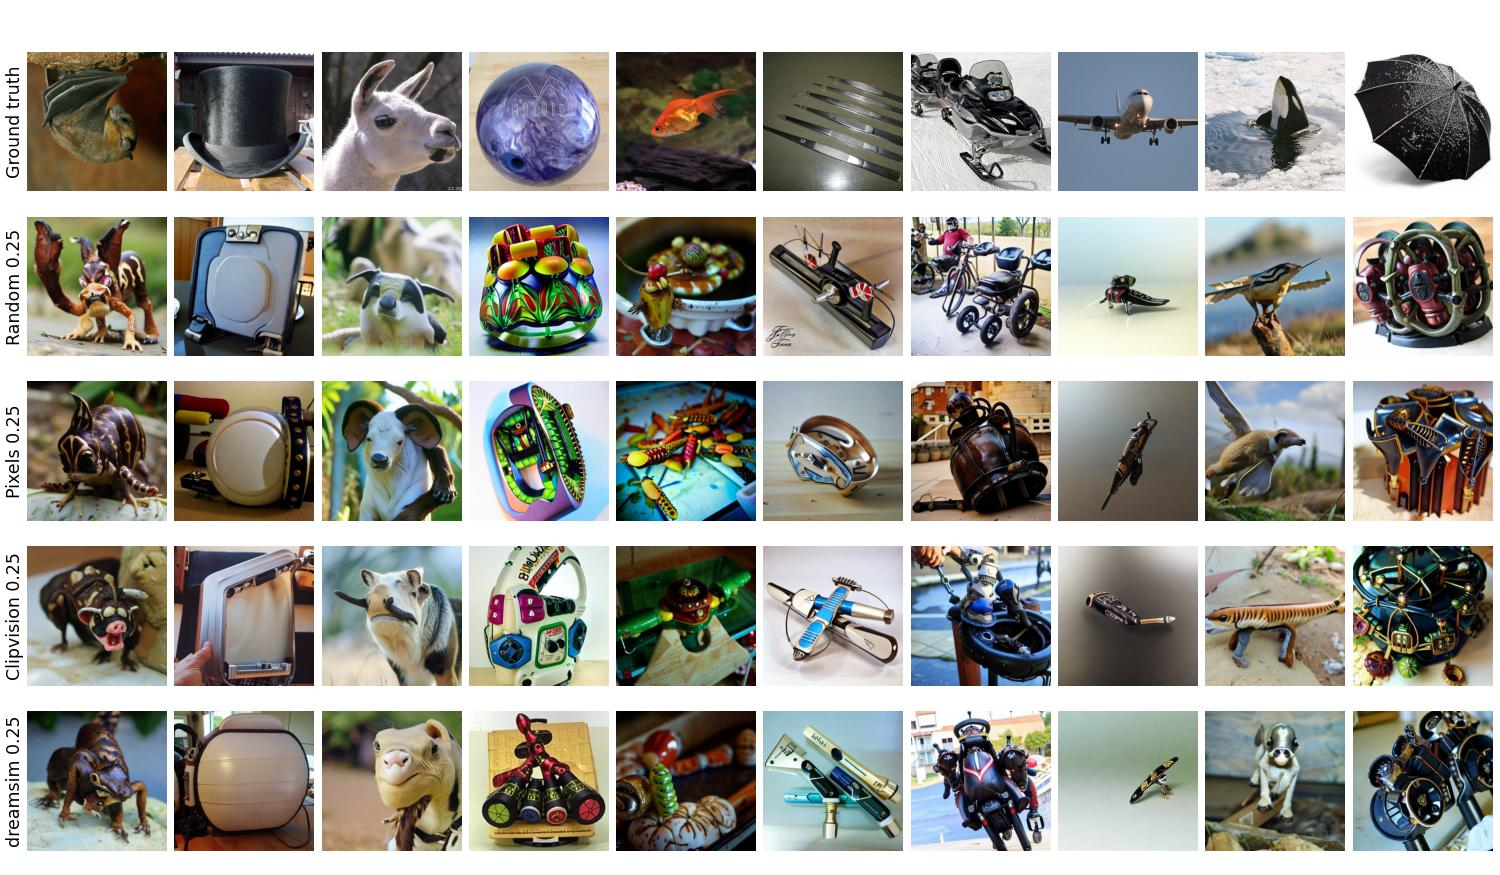
\includegraphics[width=1\textwidth]{plots/dropout_qual_eval_bd_test.JPEG}
   \caption{A nice image}\label{fig:dropout_qual_eval_bd_test}
\end{figure}

\begin{figure}[ht]
   \centering
   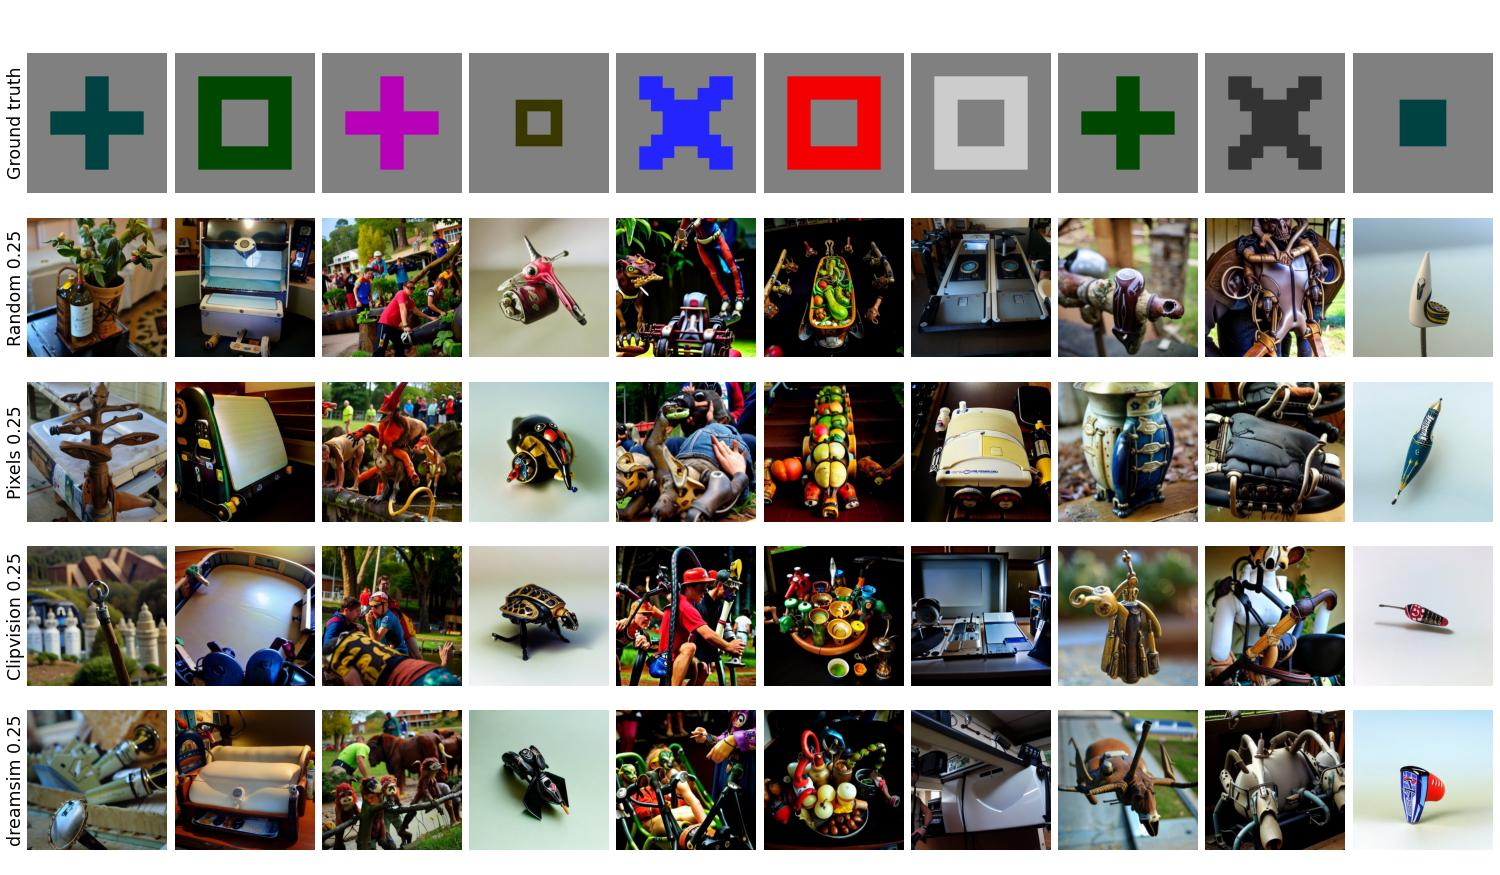
\includegraphics[width=1\textwidth]{plots/dropout_qual_eval_bd_art.JPEG}
   \caption{A nice image}\label{fig:dropout_qual_eval_bd_art}
\end{figure}

\section{Ai Captions}
\begin{figure}[ht]
   \centering
   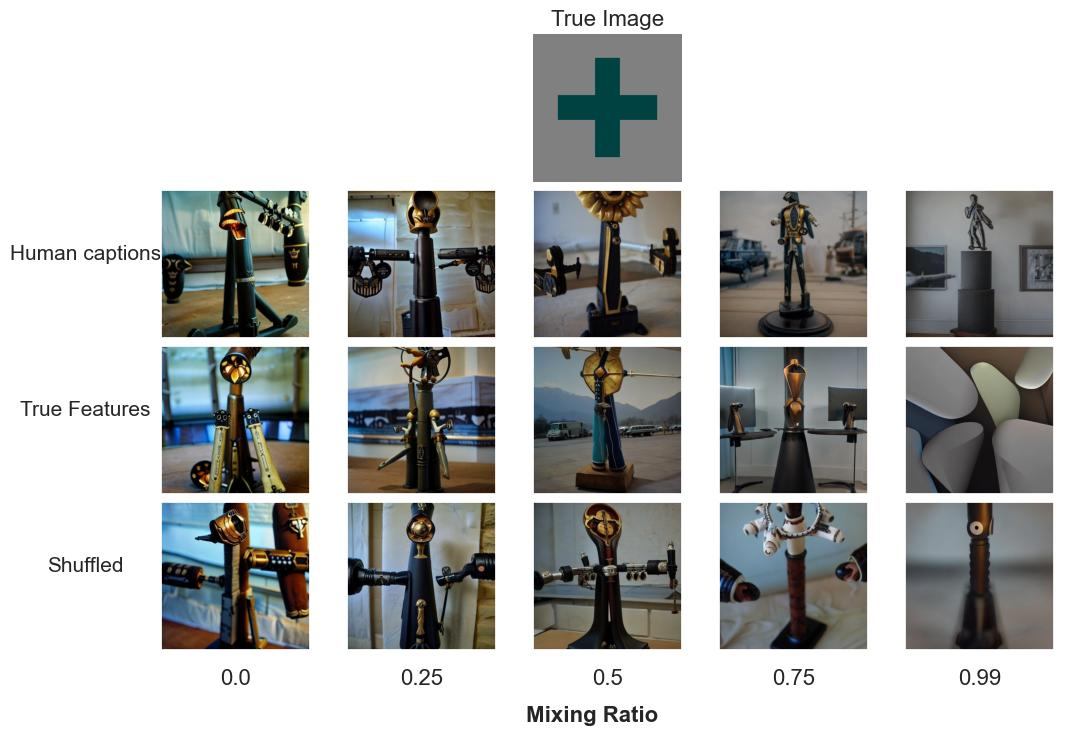
\includegraphics[width=1\textwidth]{plots/aicap_reconstruction_evolution_art_0.JPEG}
   \caption{AI-cap Reconstructions Artificial Shapes}\label{fig:aicap_reconstruction_evolution_art_0}
\end{figure}

\begin{figure}[ht]
   \centering
   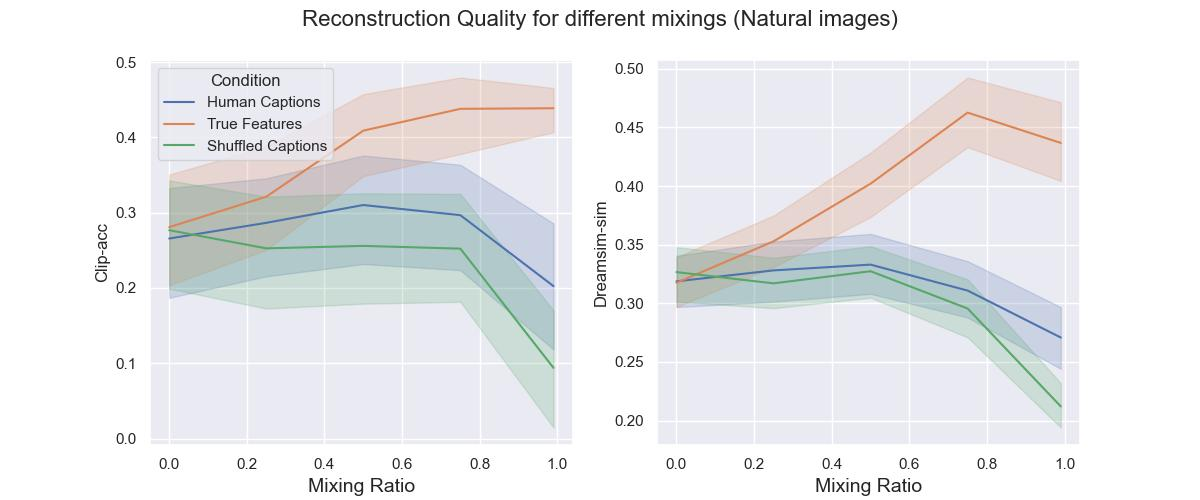
\includegraphics[width=1\textwidth]{plots/aicap_reconstruction_quant_evolution_test.JPEG}
   \caption{AI-cap Reconstructions Artificial Shapes}\label{fig:aicap_reconstruction_quant_evolution_test}
\end{figure}

\begin{figure}[ht]
   \centering
   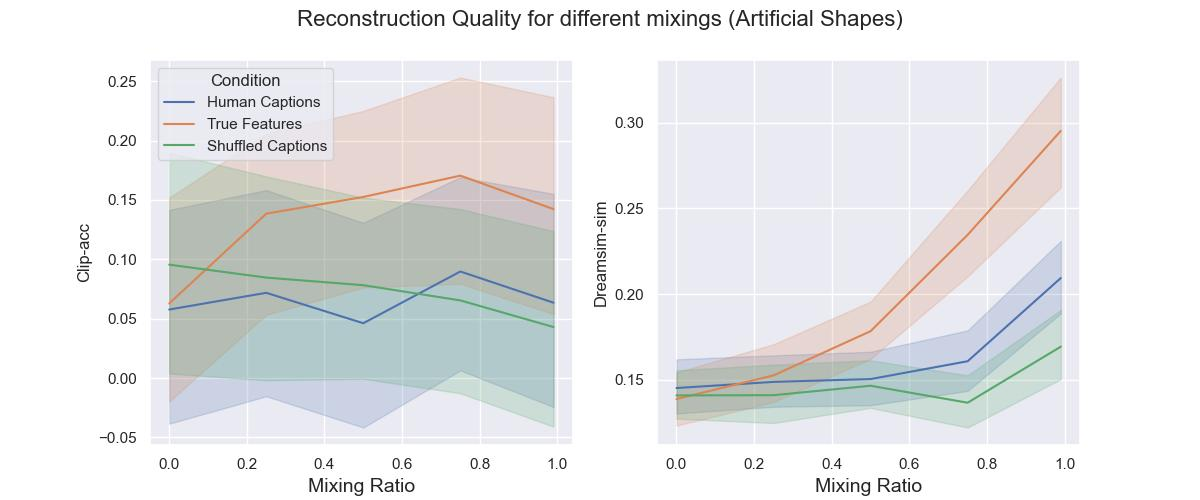
\includegraphics[width=1\textwidth]{plots/aicap_reconstruction_quant_evolution_art.JPEG}
   \caption{AI-cap Reconstructions Artificial Shapes}\label{fig:aicap_reconstruction_quant_evolution_art}
\end{figure}

\section{Perturbations}
\begin{figure}[ht]
    \centering
    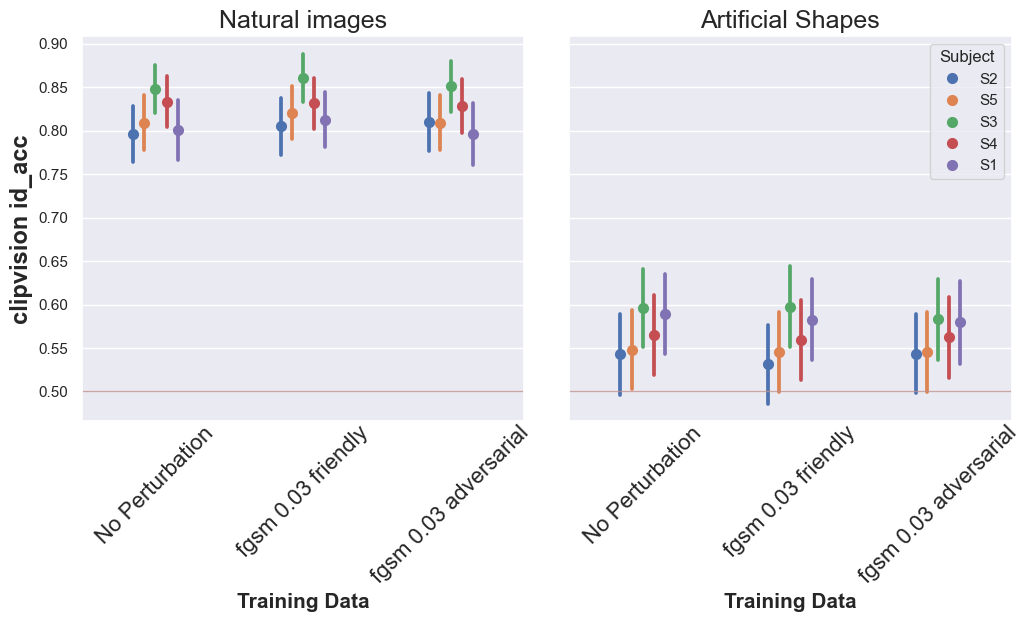
\includegraphics[width=1\textwidth]{plots/advpert_translator_fgsm_0.03.png}
    \caption{A nice image}\label{fig:advpert_translator_fgsm_0}
\end{figure}


\begin{figure}[ht]
    \centering
    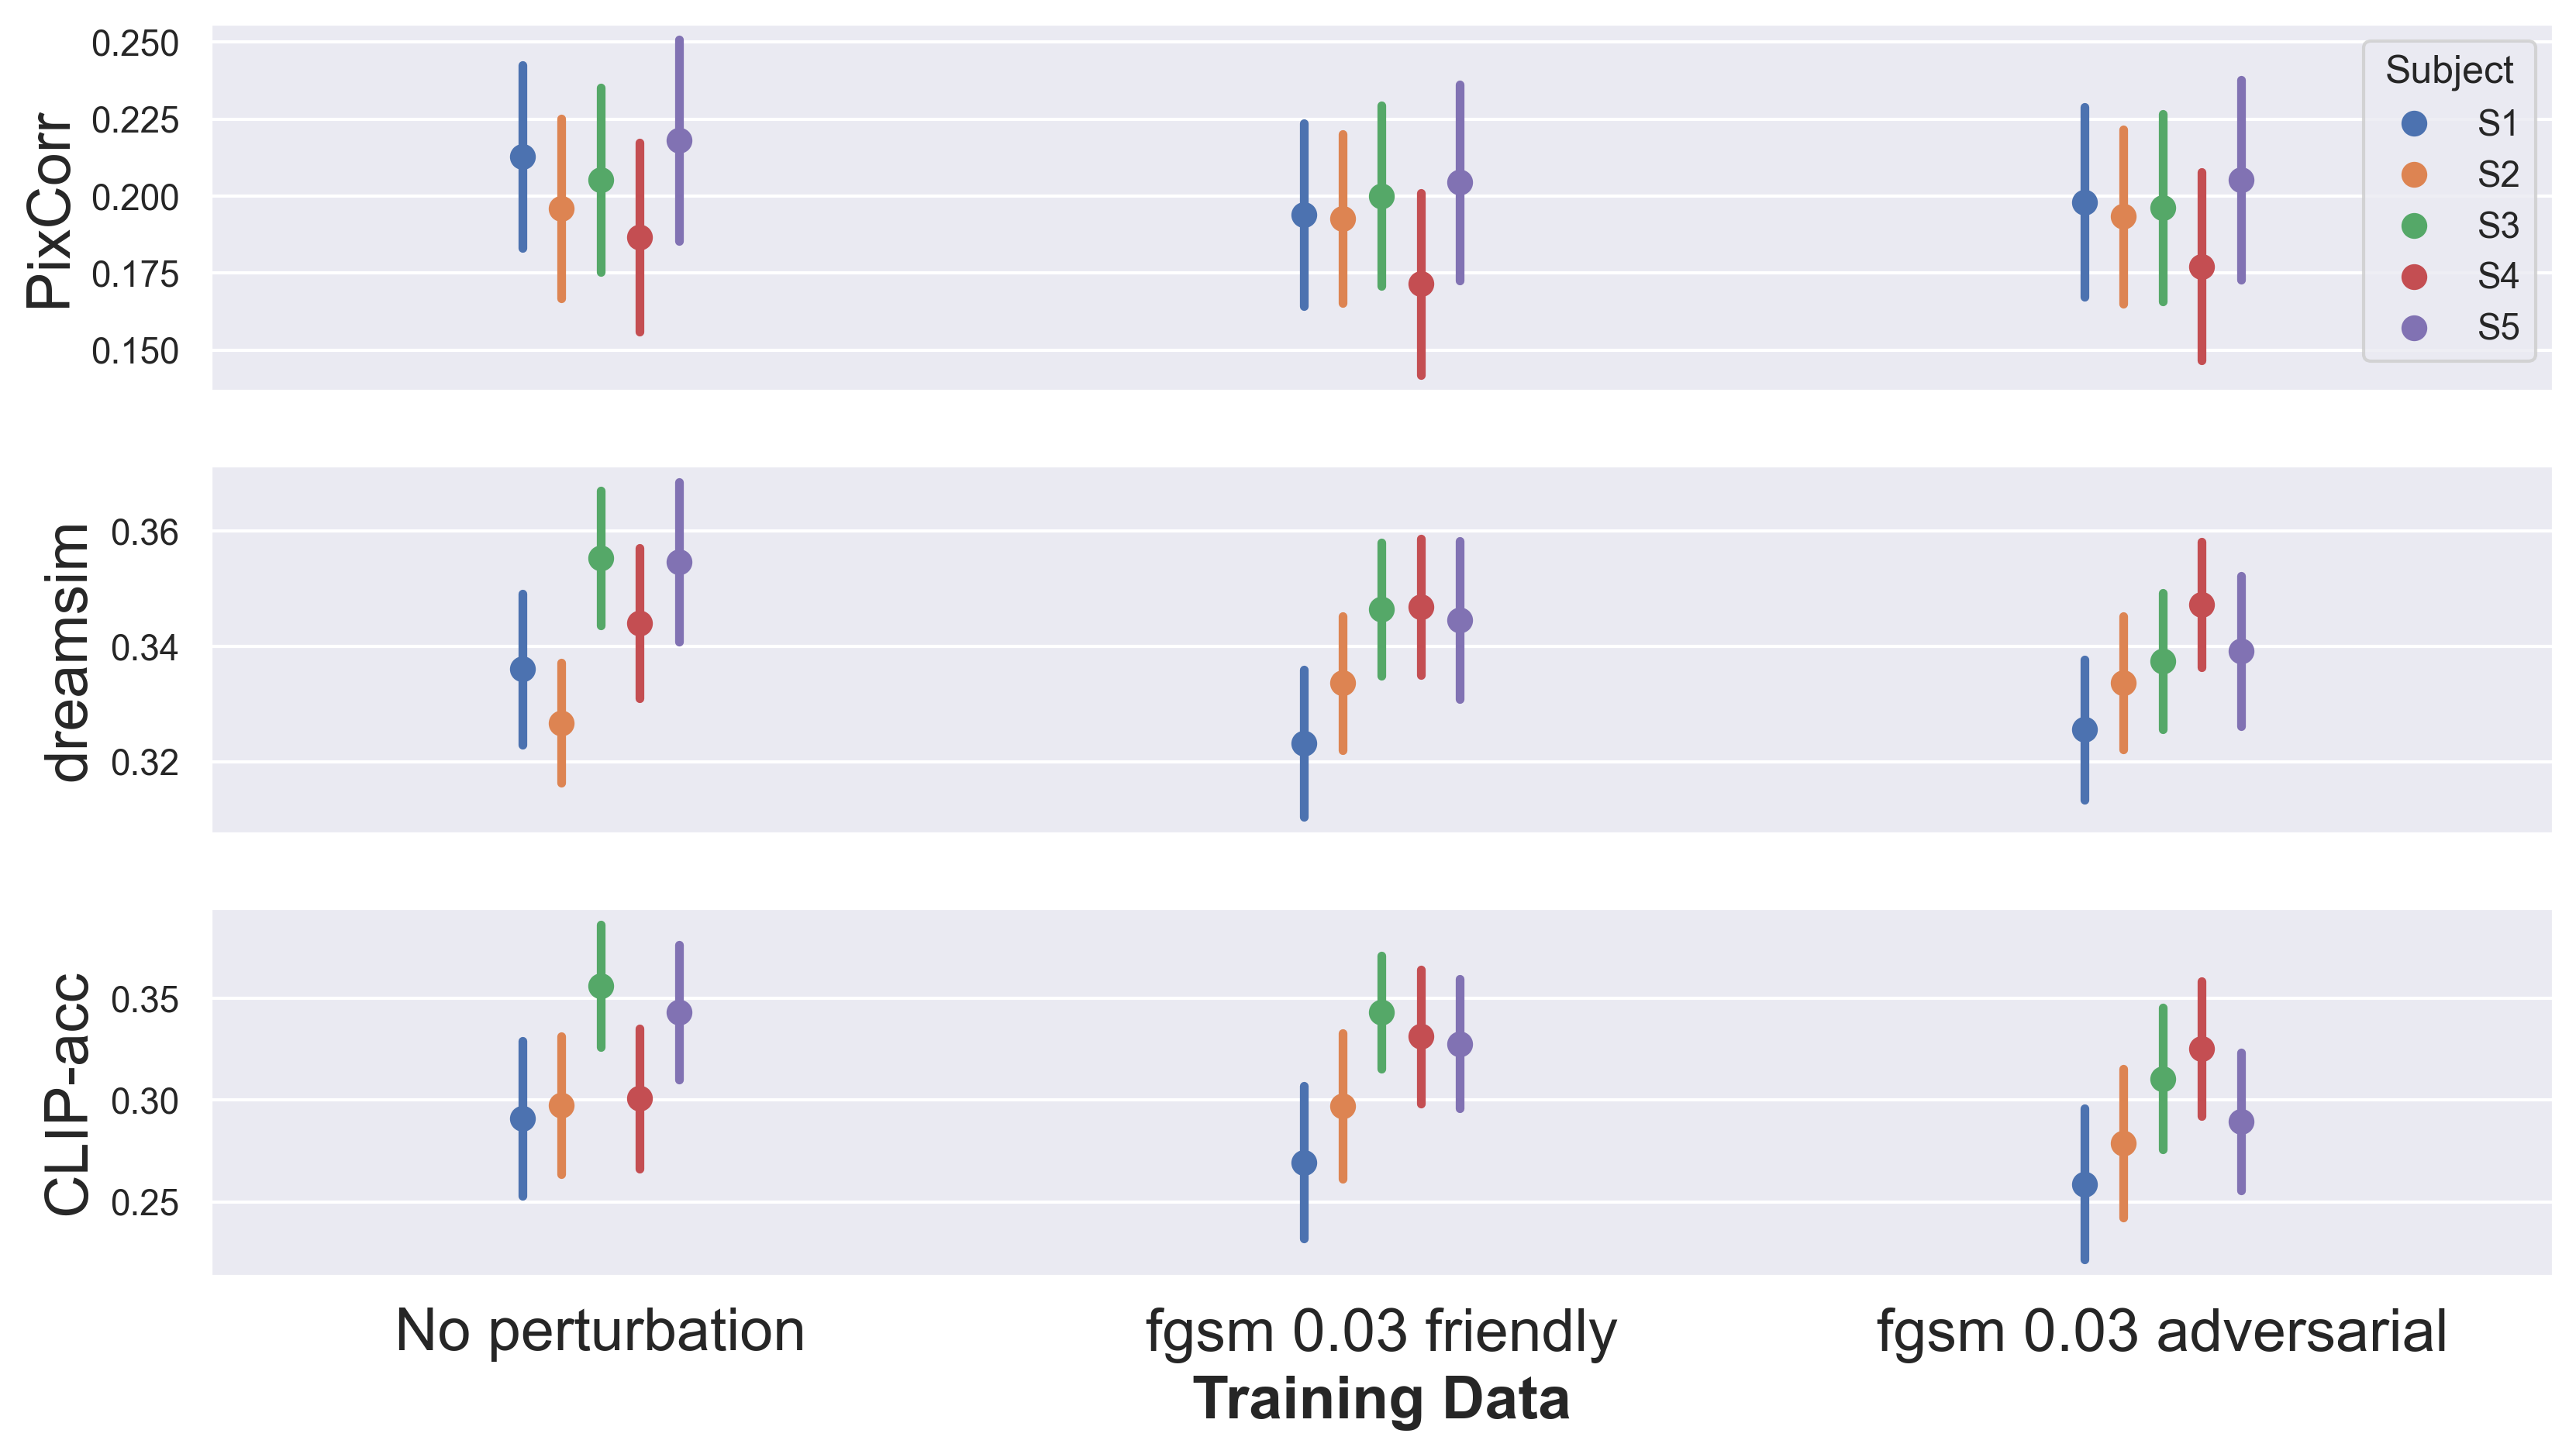
\includegraphics[width=1\textwidth]{plots/advpert_reconstruction_test_fgsm_0.03.png}
    \caption{A nice image}\label{fig:advpert_reconstruction_test_fgsm_0.03}
\end{figure}

\begin{figure}[ht]
    \centering
    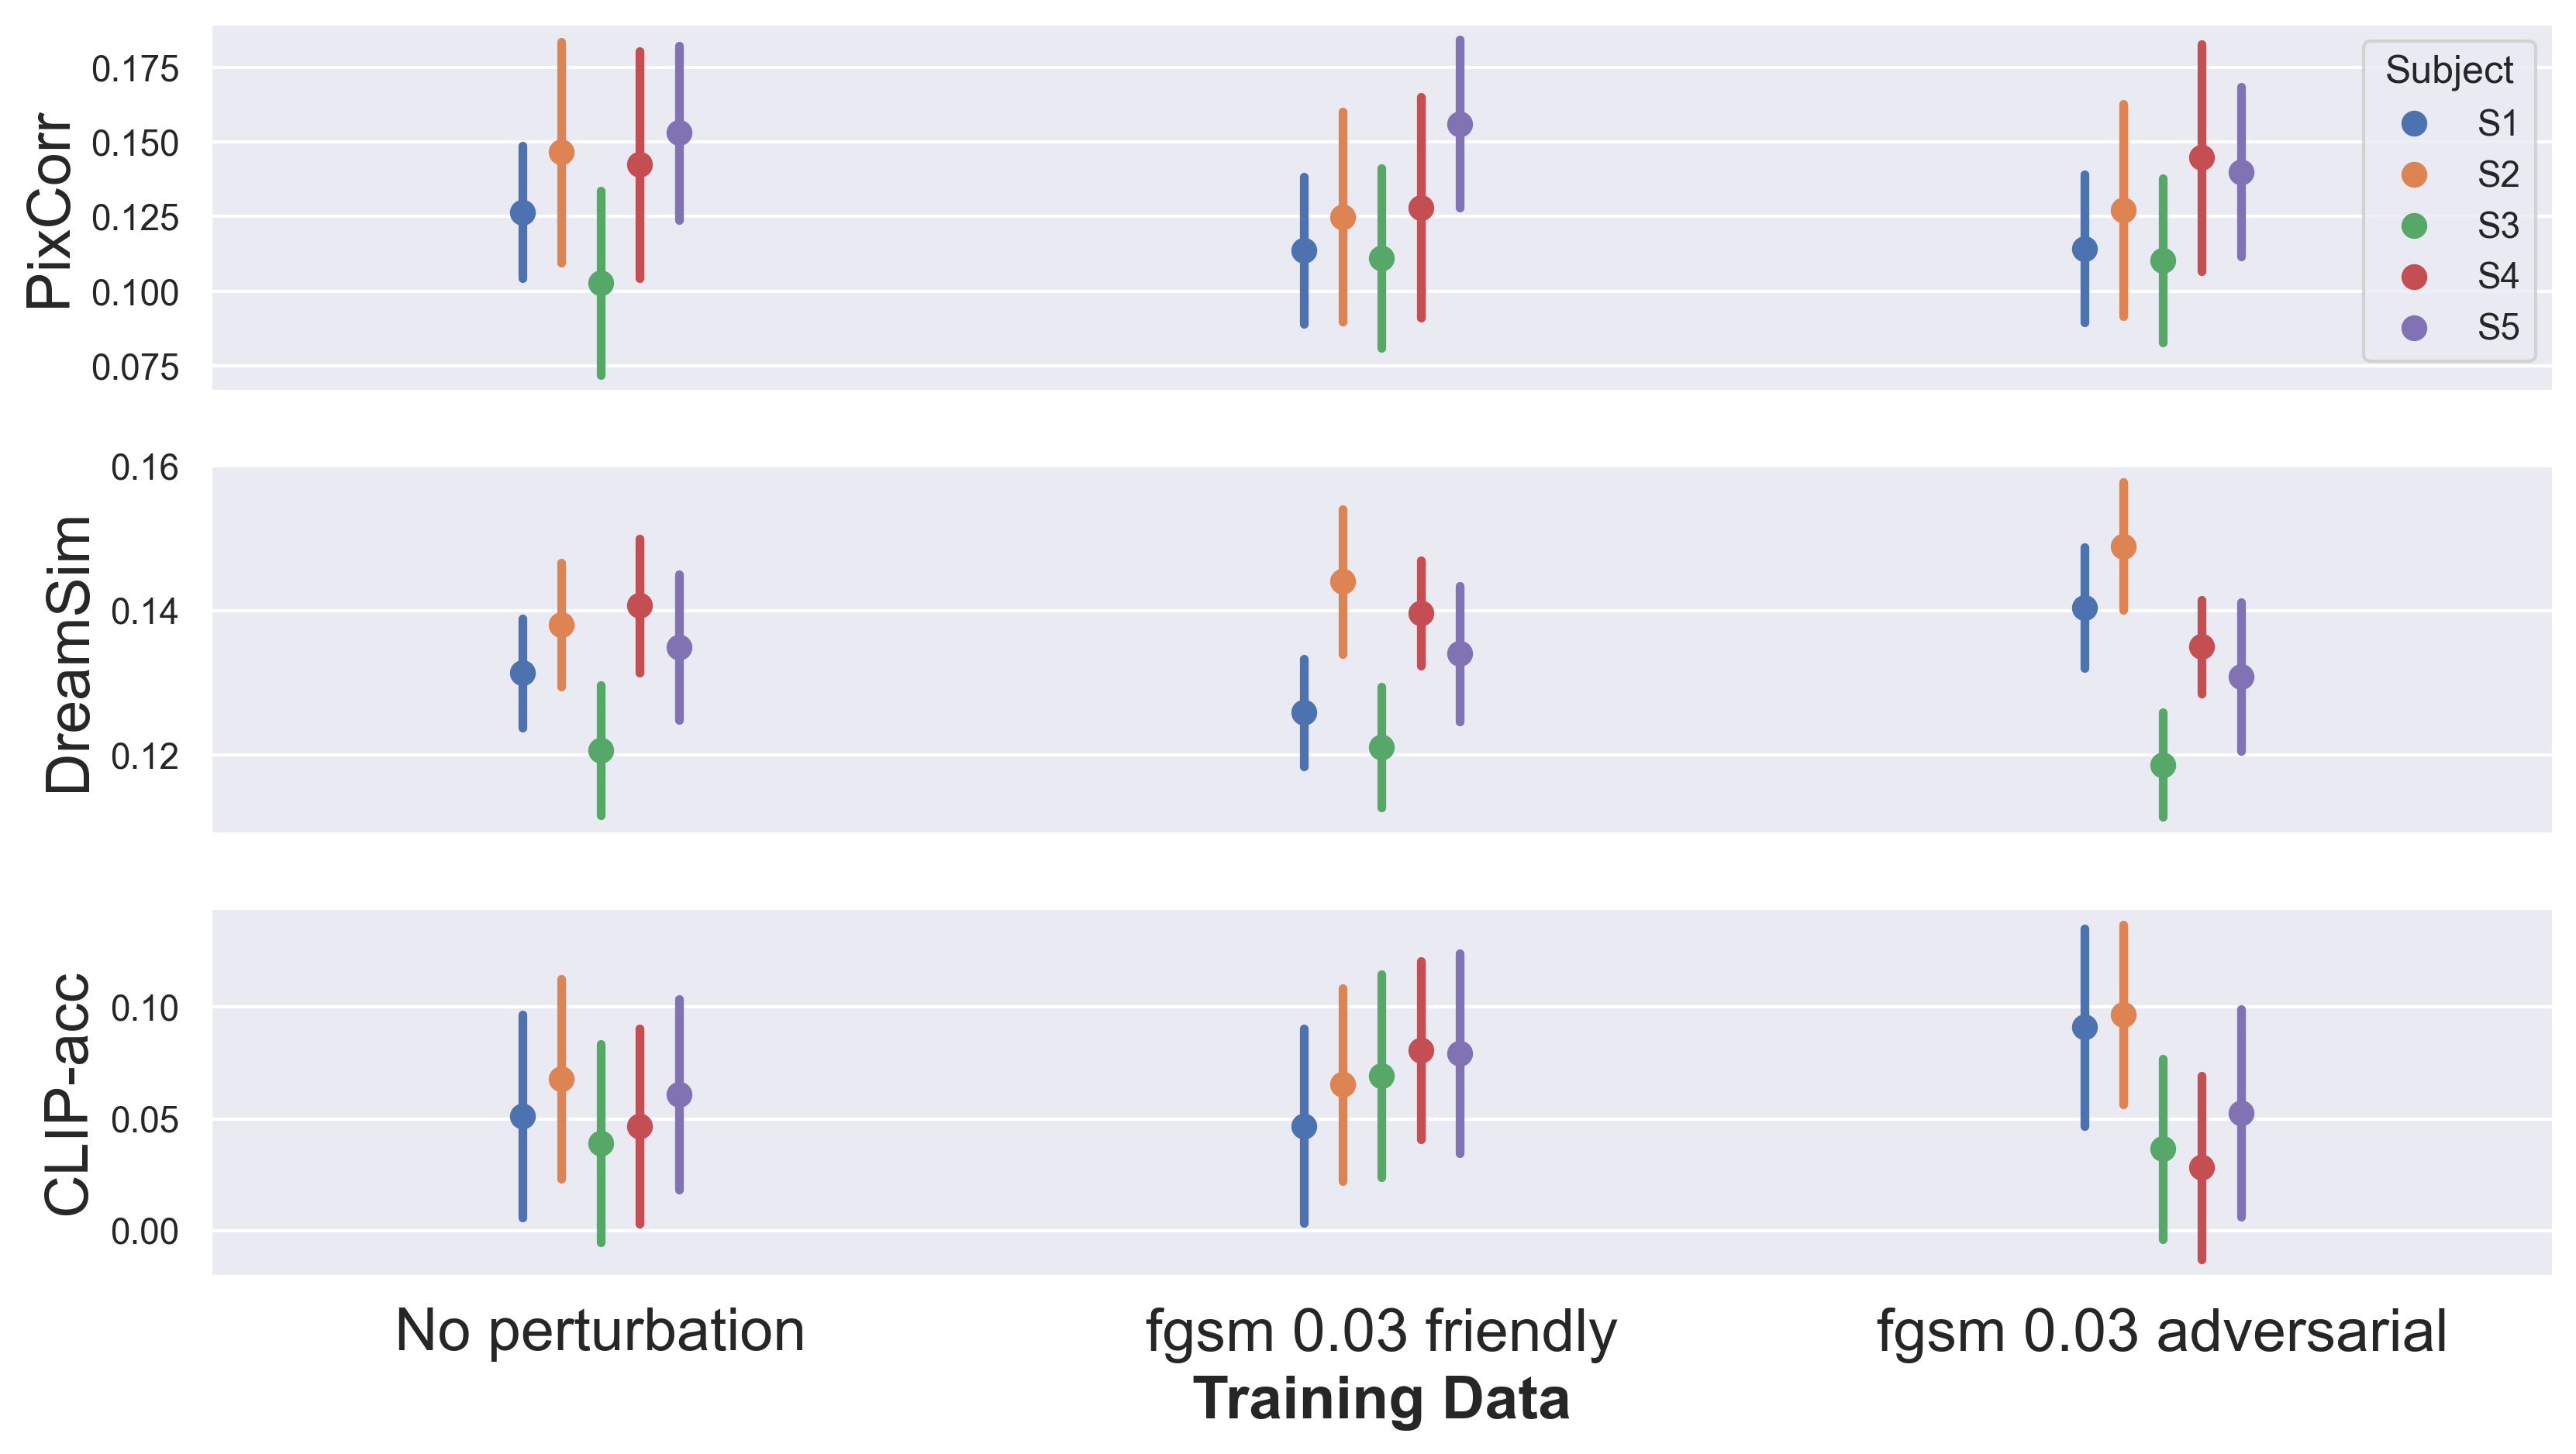
\includegraphics[width=1\textwidth]{plots/advpert_reconstruction_art_fgsm_0.03.png}
    \caption{A nice image}\label{fig:advpert_reconstruction_art_fgsm_0.03}
\end{figure}


% \chapter{Code listing}

% This example uses the \texttt{listings} package.

% \bigskip

% \lstdefinestyle{mystyle}{
%     backgroundcolor=\color{CadetBlue!15!white},   
%     commentstyle=\color{Red3},
%     numberstyle=\tiny\color{gray},
%     stringstyle=\color{Blue3},
%     basicstyle=\small\ttfamily,
%     breakatwhitespace=false,         
%     breaklines=true,                 
%     numbers=left,                    
%     numbersep=5pt,                  
%     showspaces=false,                
%     showstringspaces=false,
%     showtabs=false,                  
%     tabsize=2
% }%
% \lstset{language=[5.3]Lua,style={mystyle}}%

% \begin{lstlisting}
% function print_rate(kappa,xMin,xMax,npoints,option)
%      local c = 1-kappa*kappa
%      local croot = (1-kappa*kappa)^(1/2)
%      local logx = math.log(xMin)
%      local psi = 0
     
%      local xstep = (math.log(xMax)-math.log(xMin))/(npoints-1)
     
%      arg0 = math.sqrt(xMin/c)
%      psi0 = (1/c)*math.exp((kappa*arg0)^2)*(erfc(kappa*arg0)-erfc(arg0))
     
%      if option~=[[]] then
%   		 tex.sprint("\\addplot+["..option.."] coordinates{") 
%   		 -- addplot+ for color cycle to work
%      else
%   		 tex.sprint("\\addplot+ coordinates{")
%      end
%      tex.sprint("("..xMin..","..psi0..")")
     
%      for i=1, (npoints-1) do
%   		 x = math.exp(logx + xstep)
%   		 arg = math.sqrt(x/c)
%   		 karg = kappa*arg
%   		 if karg<5 then 
% 		 -- this break compensates for exp(karg^2), which multiplies the error in the erf approximation...
%   		    logpsi = -math.log(croot) + karg^2 + math.log(erfc(karg)-erfc(arg))
%   		    psi = math.exp(logpsi)
%   		 else
%   		    psi = (1/(karg) - 1/(2*(karg^3)) + 3/(4*(arg^5)) )/(1.77245385*croot)
%   		    -- this is the large x asymptote of the reaction rate
%   		 end
%   		 logx = math.log(x)
%   		 tex.sprint("("..x..","..psi..")")
%      end
%      tex.sprint("}")
% end
% \end{luacode*}
% \end{lstlisting}

% %% MIT Thesis class sample appendix with a long table
%% version 1.02, 2024/09/07

\chapter{One-term coefficients for heat conduction}

\section{A multipage table of numbers}
This example uses the \texttt{longtable} package: $\theta = A_1 f_1 \exp(-\lambda_1^2\mkern2mu\mathrm{Fo})$, $\overline{\theta} = D_1 \exp(-\lambda_1^2\mkern2mu\mathrm{Fo})$.


%% These four lines change the dcolumn to use text figures, instead of math figures.
%% The reason is that some mitthesis font sets use different typefaces for text and math
%% See: https://tex.stackexchange.com/a/376127/119566
\makeatletter
	\newcolumntype{T}[3]{>{\textfont0 =\the\font\DC@{#1}{#2}{#3}}c<{\DC@end}}
	\newcolumntype{d}[1]{T{.}{.}{#1}}% overwrites definition in root .tex file + gives warning message
\makeatother

{\footnotesize
% read documentation of longtable package for info on setting up a long table
% read documentation of array package and dcolumn package for info on column format specifiers
\renewcommand{\doublerulesep}{0pt}%
\newcolumntype{X}{>{\hspace{1ex}}c@{\hspace{2ex}}c@{\hspace{2ex}}c<{\hspace{1ex}}}%

\begin{longtable}{|||d{3.2}|X|X|X|||}

\caption{One-term coefficients for one-dimensional heat conduction with a convective boundary condition. Data follow H. D. Baehr and K. Stephan~\cite{baehr1998}.}%

\\
\hline\hline\hline
&&&&&&&&&\\[-7pt]
& \multicolumn{3}{c|}{\textsf{\textit{Plate}}} & \multicolumn{3}{c|}{\textsf{\textit{Cylinder}}} & \multicolumn{3}{c|||}{\textsf{\textit{Sphere}}}
\\ 
\cline{2-10} 
\multicolumn{1}{|||c|}{\raisebox{1.5ex}[0cm][0cm]{Bi}} 
       & $\lambda_1$\rule[0pt]{0pt}{11pt} & $A_1$ & $D_1$ & $\lambda_1$ & $A_1$ & $D_1$ & $\lambda_1$ & $A_1$ & $D_1$ 
\\  
\hline  
\endfirsthead
\caption[]{(continued)} \\
\hline\hline\hline
&&&&&&&&&\\[-7pt]
& \multicolumn{3}{c|}{\textsf{\textit{Plate}}} & \multicolumn{3}{c|}{\textsf{\textit{Cylinder}}} & \multicolumn{3}{c|||}{\textsf{\textit{Sphere}}}
\\ 
\cline{2-10}
\multicolumn{1}{|||c|}{\raisebox{1.5ex}[0cm][0cm]{Bi}} 
       & $\lambda_1$\rule[0pt]{0pt}{11pt} & $A_1$ & $D_1$ & $\lambda_1$ & $A_1$ & $D_1$ & $\lambda_1$ & $A_1$ & $D_1$ 
\\ \hline
&&&&&&&&&\\[-1ex]
\endhead
\hline\hline\hline
\endfoot
\hline\hline\hline
\endlastfoot 
0.01   & 0.09983  & 1.0017  & 1.0000  & 0.14124   & 1.0025  & 1.0000  & 0.17303  & 1.0030  & 1.0000\rule[0pt]{0pt}{15pt} \\ 
0.02   & 0.14095  & 1.0033  & 1.0000  & 0.19950   & 1.0050  & 1.0000  & 0.24446  & 1.0060  & 1.0000 \\ 
0.03   & 0.17234  & 1.0049  & 1.0000  & 0.24403   & 1.0075  & 1.0000  & 0.29910  & 1.0090  & 1.0000 \\ 
0.04   & 0.19868  & 1.0066  & 1.0000  & 0.28143   & 1.0099  & 1.0000  & 0.34503  & 1.0120  & 1.0000 \\  
0.05   & 0.22176  & 1.0082  & 0.9999  & 0.31426   & 1.0124  & 0.9999  & 0.38537  & 1.0150  & 1.0000 \\  
0.06   & 0.24253  & 1.0098  & 0.9999  & 0.34383   & 1.0148  & 0.9999  & 0.42173  & 1.0179  & 0.9999 \\   
0.07   & 0.26153  & 1.0114  & 0.9999  & 0.37092   & 1.0173  & 0.9999  & 0.45506  & 1.0209  & 0.9999 \\  
0.08   & 0.27913  & 1.0130  & 0.9999  & 0.39603   & 1.0197  & 0.9999  & 0.48600  & 1.0239  & 0.9999 \\  
0.09   & 0.29557  & 1.0145  & 0.9998  & 0.41954   & 1.0222  & 0.9998  & 0.51497  & 1.0268  & 0.9999 \\  
0.10   & 0.31105  & 1.0161  & 0.9998  & 0.44168   & 1.0246  & 0.9998  & 0.54228  & 1.0298  & 0.9998 \\[6pt]   
%
0.15   & 0.37788  & 1.0237  & 0.9995  & 0.53761   & 1.0365  & 0.9995  & 0.66086  & 1.0445  & 0.9996 \\*  
0.20   & 0.43284  & 1.0311  & 0.9992  & 0.61697   & 1.0483  & 0.9992  & 0.75931  & 1.0592  & 0.9993 \\  
0.25   & 0.48009  & 1.0382  & 0.9988  & 0.68559   & 1.0598  & 0.9988  & 0.84473  & 1.0737  & 0.9990 \\  
0.30   & 0.52179  & 1.0450  & 0.9983  & 0.74646   & 1.0712  & 0.9983  & 0.92079  & 1.0880  & 0.9985 \\  
0.40   & 0.59324  & 1.0580  & 0.9971  & 0.85158   & 1.0931  & 0.9970  & 1.05279  & 1.1164  & 0.9974 \\  
0.50   & 0.65327  & 1.0701  & 0.9956  & 0.94077   & 1.1143  & 0.9954  & 1.16556  & 1.1441  & 0.9960 \\ 
0.60   & 0.70507  & 1.0814  & 0.9940  & 1.01844   & 1.1345  & 0.9936  & 1.26440  & 1.1713  & 0.9944 \\  
0.70   & 0.75056  & 1.0918  & 0.9922  & 1.08725   & 1.1539  & 0.9916  & 1.35252  & 1.1978  & 0.9925 \\  
0.80   & 0.79103  & 1.1016  & 0.9903  & 1.14897   & 1.1724  & 0.9893  & 1.43203  & 1.2236  & 0.9904 \\  
0.90   & 0.82740  & 1.1107  & 0.9882  & 1.20484   & 1.1902  & 0.9869  & 1.50442  & 1.2488  & 0.9880 \\[6pt]  
%
1.00   & 0.86033  & 1.1191  & 0.9861  & 1.25578   & 1.2071  & 0.9843  & 1.57080  & 1.2732  & 0.9855 \\* 
1.10   & 0.89035  & 1.1270  & 0.9839  & 1.30251   & 1.2232  & 0.9815  & 1.63199  & 1.2970  & 0.9828 \\  
1.20   & 0.91785  & 1.1344  & 0.9817  & 1.34558   & 1.2387  & 0.9787  & 1.68868  & 1.3201  & 0.9800 \\ 
1.30   & 0.94316  & 1.1412  & 0.9794  & 1.38543   & 1.2533  & 0.9757  & 1.74140  & 1.3424  & 0.9770 \\  
1.40   & 0.96655  & 1.1477  & 0.9771  & 1.42246   & 1.2673  & 0.9727  & 1.79058  & 1.3640  & 0.9739 \\  
1.50   & 0.98824  & 1.1537  & 0.9748  & 1.45695   & 1.2807  & 0.9696  & 1.83660  & 1.3850  & 0.9707 \\ 
1.60   & 1.00842  & 1.1593  & 0.9726  & 1.48917   & 1.2934  & 0.9665  & 1.87976  & 1.4052  & 0.9674 \\  
1.70   & 1.02725  & 1.1645  & 0.9703  & 1.51936   & 1.3055  & 0.9633  & 1.92035  & 1.4247  & 0.9640 \\* 
1.80   & 1.04486  & 1.1695  & 0.9680  & 1.54769   & 1.3170  & 0.9601  & 1.95857  & 1.4436  & 0.9605 \\*  
1.90   & 1.06136  & 1.1741  & 0.9658  & 1.57434   & 1.3279  & 0.9569  & 1.99465  & 1.4618  & 0.9570 \\[6pt]  
%
2.00   & 1.07687  & 1.1785  & 0.9635  & 1.59945   & 1.3384  & 0.9537  & 2.02876  & 1.4793  & 0.9534 \\*  
2.20   & 1.10524  & 1.1864  & 0.9592  & 1.64557   & 1.3578  & 0.9472  & 2.09166  & 1.5125  & 0.9462 \\  
2.40   & 1.13056  & 1.1934  & 0.9549  & 1.68691   & 1.3754  & 0.9408  & 2.14834  & 1.5433  & 0.9389 \\  
2.60   & 1.15330  & 1.1997  & 0.9509  & 1.72418   & 1.3914  & 0.9345  & 2.19967  & 1.5718  & 0.9316 \\  
2.80   & 1.17383  & 1.2052  & 0.9469  & 1.75794   & 1.4059  & 0.9284  & 2.24633  & 1.5982  & 0.9243 \\ 
3.00   & 1.19246  & 1.2102  & 0.9431  & 1.78866   & 1.4191  & 0.9224  & 2.28893  & 1.6227  & 0.9171 \\     
3.50   & 1.23227  & 1.2206  & 0.9343  & 1.85449   & 1.4473  & 0.9081  & 2.38064  & 1.6761  & 0.8995 \\     
4.00   & 1.26459  & 1.2287  & 0.9264  & 1.90808   & 1.4698  & 0.8950  & 2.45564  & 1.7202  & 0.8830 \\*   
4.50   & 1.29134  & 1.2351  & 0.9193  & 1.95248   & 1.4880  & 0.8830  & 2.51795  & 1.7567  & 0.8675 \\*    
5.00   & 1.31384  & 1.2402  & 0.9130  & 1.98981   & 1.5029  & 0.8721  & 2.57043  & 1.7870  & 0.8533 \\[6pt]    
%
6.00   & 1.34955  & 1.2479  & 0.9021  & 2.04901   & 1.5253  & 0.8532  & 2.65366  & 1.8338  & 0.8281 \\*     
7.00   & 1.37662  & 1.2532  & 0.8932  & 2.09373   & 1.5411  & 0.8375  & 2.71646  & 1.8673  & 0.8069 \\    
8.00   & 1.39782  & 1.2570  & 0.8858  & 2.12864   & 1.5526  & 0.8244  & 2.76536  & 1.8920  & 0.7889 \\     
9.00   & 1.41487  & 1.2598  & 0.8796  & 2.15661   & 1.5611  & 0.8133  & 2.80443  & 1.9106  & 0.7737 \\     
10.00  & 1.42887  & 1.2620  & 0.8743  & 2.17950   & 1.5677  & 0.8039  & 2.83630  & 1.9249  & 0.7607 \\     
12.00  & 1.45050  & 1.2650  & 0.8658  & 2.21468   & 1.5769  & 0.7887  & 2.88509  & 1.9450  & 0.7397 \\     
14.00  & 1.46643  & 1.2669  & 0.8592  & 2.24044   & 1.5828  & 0.7770  & 2.92060  & 1.9581  & 0.7236 \\     
16.00  & 1.47864  & 1.2683  & 0.8541  & 2.26008   & 1.5869  & 0.7678  & 2.94756  & 1.9670  & 0.7109 \\*     
18.00  & 1.48830  & 1.2692  & 0.8499  & 2.27556   & 1.5898  & 0.7603  & 2.96871  & 1.9734  & 0.7007 \\*     
20.00  & 1.49613  & 1.2699  & 0.8464  & 2.28805   & 1.5919  & 0.7542  & 2.98572  & 1.9781  & 0.6922 \\[6pt]     
%
25.00  & 1.51045  & 1.2710  & 0.8400  & 2.31080   & 1.5954  & 0.7427  & 3.01656  & 1.9856  & 0.6766 \\*     
30.00  & 1.52017  & 1.2717  & 0.8355  & 2.32614   & 1.5973  & 0.7348  & 3.03724  & 1.9898  & 0.6658 \\     
35.00  & 1.52719  & 1.2721  & 0.8322  & 2.33719   & 1.5985  & 0.7290  & 3.05207  & 1.9924  & 0.6579 \\     
40.00  & 1.53250  & 1.2723  & 0.8296  & 2.34552   & 1.5993  & 0.7246  & 3.06321  & 1.9942  & 0.6519 \\    
50.00  & 1.54001  & 1.2727  & 0.8260  & 2.35724   & 1.6002  & 0.7183  & 3.07884  & 1.9962  & 0.6434 \\     
60.00  & 1.54505  & 1.2728  & 0.8235  & 2.36510   & 1.6007  & 0.7140  & 3.08928  & 1.9974  & 0.6376 \\     
80.00  & 1.55141  & 1.2730  & 0.8204  & 2.37496   & 1.6013  & 0.7085  & 3.10234  & 1.9985  & 0.6303 \\    
100.00 & 1.55525  & 1.2731  & 0.8185  & 2.38090   & 1.6015  & 0.7052  & 3.11019  & 1.9990  & 0.6259 \\*    
200.00 & 1.56298  & 1.2732  & 0.8146  & 2.39283   & 1.6019  & 0.6985  & 3.12589  & 1.9998  & 0.6170 \\*    
\infty & 1.57080  & 1.2732  & 0.8106  & 2.40483   & 1.6020  & 0.6917  & 3.14159  & 2.0000  & 0.6079 \\[3pt] 
\end{longtable}
}


%%% Bibliography (biblatex)  %%%%%%%%%%%%%%%%%%%%%%%%%%%%%%%%%%%%%%%%%%%%%%%%%%%%%%%%%%%%%%%%%%%%%%

\defbibheading{bibintoc}{\chapter*{#1}\addcontentsline{toc}{backmatter}{\refname}} 
% this sets the title of contents name for bibliography to \refname (= References)
% change "backmatter" to "chapter" if you prefer a bold face entry in the table of contents

\printbibliography[title={\refname},heading=bibintoc]

% biblatex also supports chapter-by-chapter bibliography, https://tex.stackexchange.com/a/296502/119566
% see the biblatex manual, section 3.14.3


%%%% Option for natbib %%%%%%%%%%%%%

%%   use an appropriate style (.bst) and your own .bib file[s]

%\bibliographystyle{plainnat}
%\bibliography{mitthesis-sample.bib}

\end{document} 
 